\documentclass[12pt, letterpaper]{article}
\usepackage[margin=1in]{geometry}
\usepackage{mathptmx}
\usepackage{amsmath}
\usepackage{graphicx}
\usepackage{booktabs}
\usepackage{multirow}
\usepackage[font={small,it}, justification=centering, labelfont=bf]{caption}
\usepackage{float}
\usepackage[skip=4pt]{parskip}
\usepackage{hyperref}
\hypersetup{colorlinks=true, linkcolor=blue, urlcolor=blue}
\usepackage{titlesec}
\titlespacing*{\section}{0pt}{8pt}{4pt}
\titlespacing*{\subsection}{0pt}{6pt}{2pt}

% Roman numeral section counter
\renewcommand{\thesection}{\Roman{section}}
\titleformat{\section}{\normalfont\bfseries\large}{\thesection.}{0.5em}{}

% Simple arabic numbering for subsections (1. 2. 3. not III.1)
\renewcommand{\thesubsection}{\arabic{subsection}}
\titleformat{\subsection}{\normalfont\bfseries}{\thesubsection.}{0.5em}{}

\begin{document}

\begin{center}
  {\large \textbf{Report for CDA 3201L Lab \#6}}\\[2pt]
  {\large \textbf{Sequential Circuits -- Game Show Circuit}}\\[8pt]
  \begin{tabular}{ll}
    \textbf{Name:} Tuan Khang Phan & \textbf{UID:} U30382645 \\
    \textbf{Name:} Huu Phat Nguyen & \textbf{UID:} U46082380 \\
  \end{tabular}
\end{center}

\section{Introduction}

The purpose of this lab is to gain a deeper understanding of sequential circuit design by building a game show circuit. The circuit determines which of two contestants ``rings in'' first to answer a question. This lab also introduces configuring and using function generators to provide the clock signal for the circuit. The design uses D flip-flops (DFFs) to store state and combinational logic to compute the next state based on contestant inputs.

\section{Methods and Materials}

We used the following components and equipment:

\begin{itemize}
  \item 74LS74 dual positive edge-triggered D flip-flop IC
  \item 74LS08 quad 2-input AND gate IC
  \item 74LS32 quad 2-input OR gate IC
  \item 74LS04 hex inverter IC
  \item Breadboard and jumper wires
  \item Two LEDs and resistors
  \item Two push buttons (for contestant inputs $X_1$ and $X_0$)
  \item 5\,V DC power supply
  \item Function generator (for the clock signal)
  \item Oscilloscope
\end{itemize}

First, we derived the state transition table and excitation equations from the lab specification. We then filled in the Karnaugh maps for $Q_0^*$ and $Q_1^*$ and simplified the expressions. Using the 74LS74 datasheet, we identified the pin-out for the DFFs, including the asynchronous clear (CLR) pin used for reset. We configured the function generator to output a square wave at an appropriate frequency and amplitude to serve as the clock. The circuit was wired on the breadboard, connecting the combinational logic for the D inputs of each flip-flop, the clock from the function generator, and the reset via the CLR pins. The Q outputs of the flip-flops were connected directly to LEDs through current-limiting resistors.

\section{Results}

\subsection{State Transition Diagram and K-map for $Q_1^*$}

The game show circuit has four states:

\begin{itemize}
  \item \textbf{State A} ($Q_1Q_0 = 00$): Wait state. No contestant has rung in. Both LEDs are off ($Y_1Y_0 = 00$).
  \item \textbf{State B} ($Q_1Q_0 = 01$): Contestant 0 wins. LED0 is on ($Y_1Y_0 = 01$).
  \item \textbf{State C} ($Q_1Q_0 = 10$): Contestant 1 wins. LED1 is on ($Y_1Y_0 = 10$).
  \item \textbf{State D} ($Q_1Q_0 = 11$): Tie. Both LEDs are on ($Y_1Y_0 = 11$).
\end{itemize}

The state transition table is:

\begin{center}
  \begin{tabular}{|c|cccc|c|}
    \hline
    & \multicolumn{4}{c|}{NS ($Q_1^*Q_0^*$) for Input $X_1X_0$} & \\
    PS ($Q_1Q_0$) & 00 & 01 & 10 & 11 & $Y_1Y_0$ \\
    \hline
    A = 00 & A & B & C & D & 00 \\
    B = 01 & B & B & B & B & 01 \\
    C = 10 & C & C & C & C & 10 \\
    D = 11 & D & D & D & D & 11 \\
    \hline
  \end{tabular}
\end{center}

From the state transition table, the K-map for $Q_1^*$ is:

\begin{center}
  \begin{tabular}{|c|c|cccc|}
    \hline
    \multicolumn{2}{|c|}{$Q_1^*$} & \multicolumn{4}{c|}{$X_1X_0$} \\
    \multicolumn{2}{|c|}{} & 00 & 01 & 11 & 10 \\
    \hline
    \multirow{4}{*}{$Q_1Q_0$} & 00 & 0 & 0 & 1 & 1 \\
    & 01 & 0 & 0 & 0 & 0 \\
    & 11 & 1 & 1 & 1 & 1 \\
    & 10 & 1 & 1 & 1 & 1 \\
    \hline
  \end{tabular}
\end{center}

Grouping the 1s in the K-map:
\begin{itemize}
  \item The four cells in rows $Q_1Q_0 = 10$ and $Q_1Q_0 = 11$ form a group of 8, giving the term $Q_1$.
  \item The two cells at $Q_1Q_0 = 00$, $X_1X_0 = 10$ and $Q_1Q_0 = 00$, $X_1X_0 = 11$ combine with the corresponding cells in row 10, giving the term $X_1 \cdot \overline{Q_0}$.
\end{itemize}

The simplified excitation equation is:
\[
  Q_1^* = Q_1 + X_1 \cdot \overline{Q_0}
\]

For reference, the K-map for $Q_0^*$ (derived in the prelab) yields:
\[
  Q_0^* = Q_0 + X_0 \cdot \overline{Q_1}
\]

Since the DFF characteristic equation is $Q^* = D$, the excitation equations become:
\begin{align*}
  D_0 &= Q_0 + X_0 \cdot \overline{Q_1} \\
  D_1 &= Q_1 + X_1 \cdot \overline{Q_0}
\end{align*}

The output equations are simply:
\begin{align*}
  Y_0 &= Q_0 \\
  Y_1 &= Q_1
\end{align*}

\subsection{Discussion of Expected Circuit Behavior}

The circuit begins in the wait state (State A) after reset is asserted via the CLR pin on the 74LS74. In this state, both flip-flop outputs are 0, so both LEDs are off. The circuit samples the inputs $X_1$ and $X_0$ on each rising clock edge.

If contestant 0 presses their button first ($X_1X_0 = 01$), the next-state logic computes $D_0 = 0 + 1 \cdot 1 = 1$ and $D_1 = 0 + 0 \cdot 1 = 0$, so on the next clock edge the circuit transitions to State B ($Q_1Q_0 = 01$). LED0 turns on. Once in State B, $Q_0 = 1$, so $D_0 = 1 + \ldots = 1$ regardless of inputs, and $D_1 = 0 + X_1 \cdot \overline{Q_0} = 0 + X_1 \cdot 0 = 0$ regardless of $X_1$. The circuit is locked in State B until reset.

Symmetrically, if contestant 1 presses first ($X_1X_0 = 10$), the circuit moves to State C ($Q_1Q_0 = 10$), lighting LED1 and locking out further input changes.

If both contestants press simultaneously ($X_1X_0 = 11$), the circuit transitions to State D ($Q_1Q_0 = 11$), both LEDs light up indicating a tie, and the circuit locks in this state.

In all non-wait states (B, C, D), the excitation equations ensure that the present state bits that are already 1 remain 1, and the bits that are 0 cannot become 1 because the corresponding input term is multiplied by the complement of the other state bit (which is already 1). This is what makes the circuit ``lock'' once a winner is determined.

To return to the wait state, the asynchronous CLR input on the 74LS74 is asserted (active low), which forces both flip-flop outputs to 0 regardless of the clock or D inputs.

\subsection{Physical Circuit Testing}

The circuit was built on a breadboard using the 74LS74 DFF IC along with AND, OR, and inverter gate ICs. The function generator was connected to the clock input of both flip-flops, and an oscilloscope probe was used to verify the clock signal.

\begin{figure}[H]
\centering
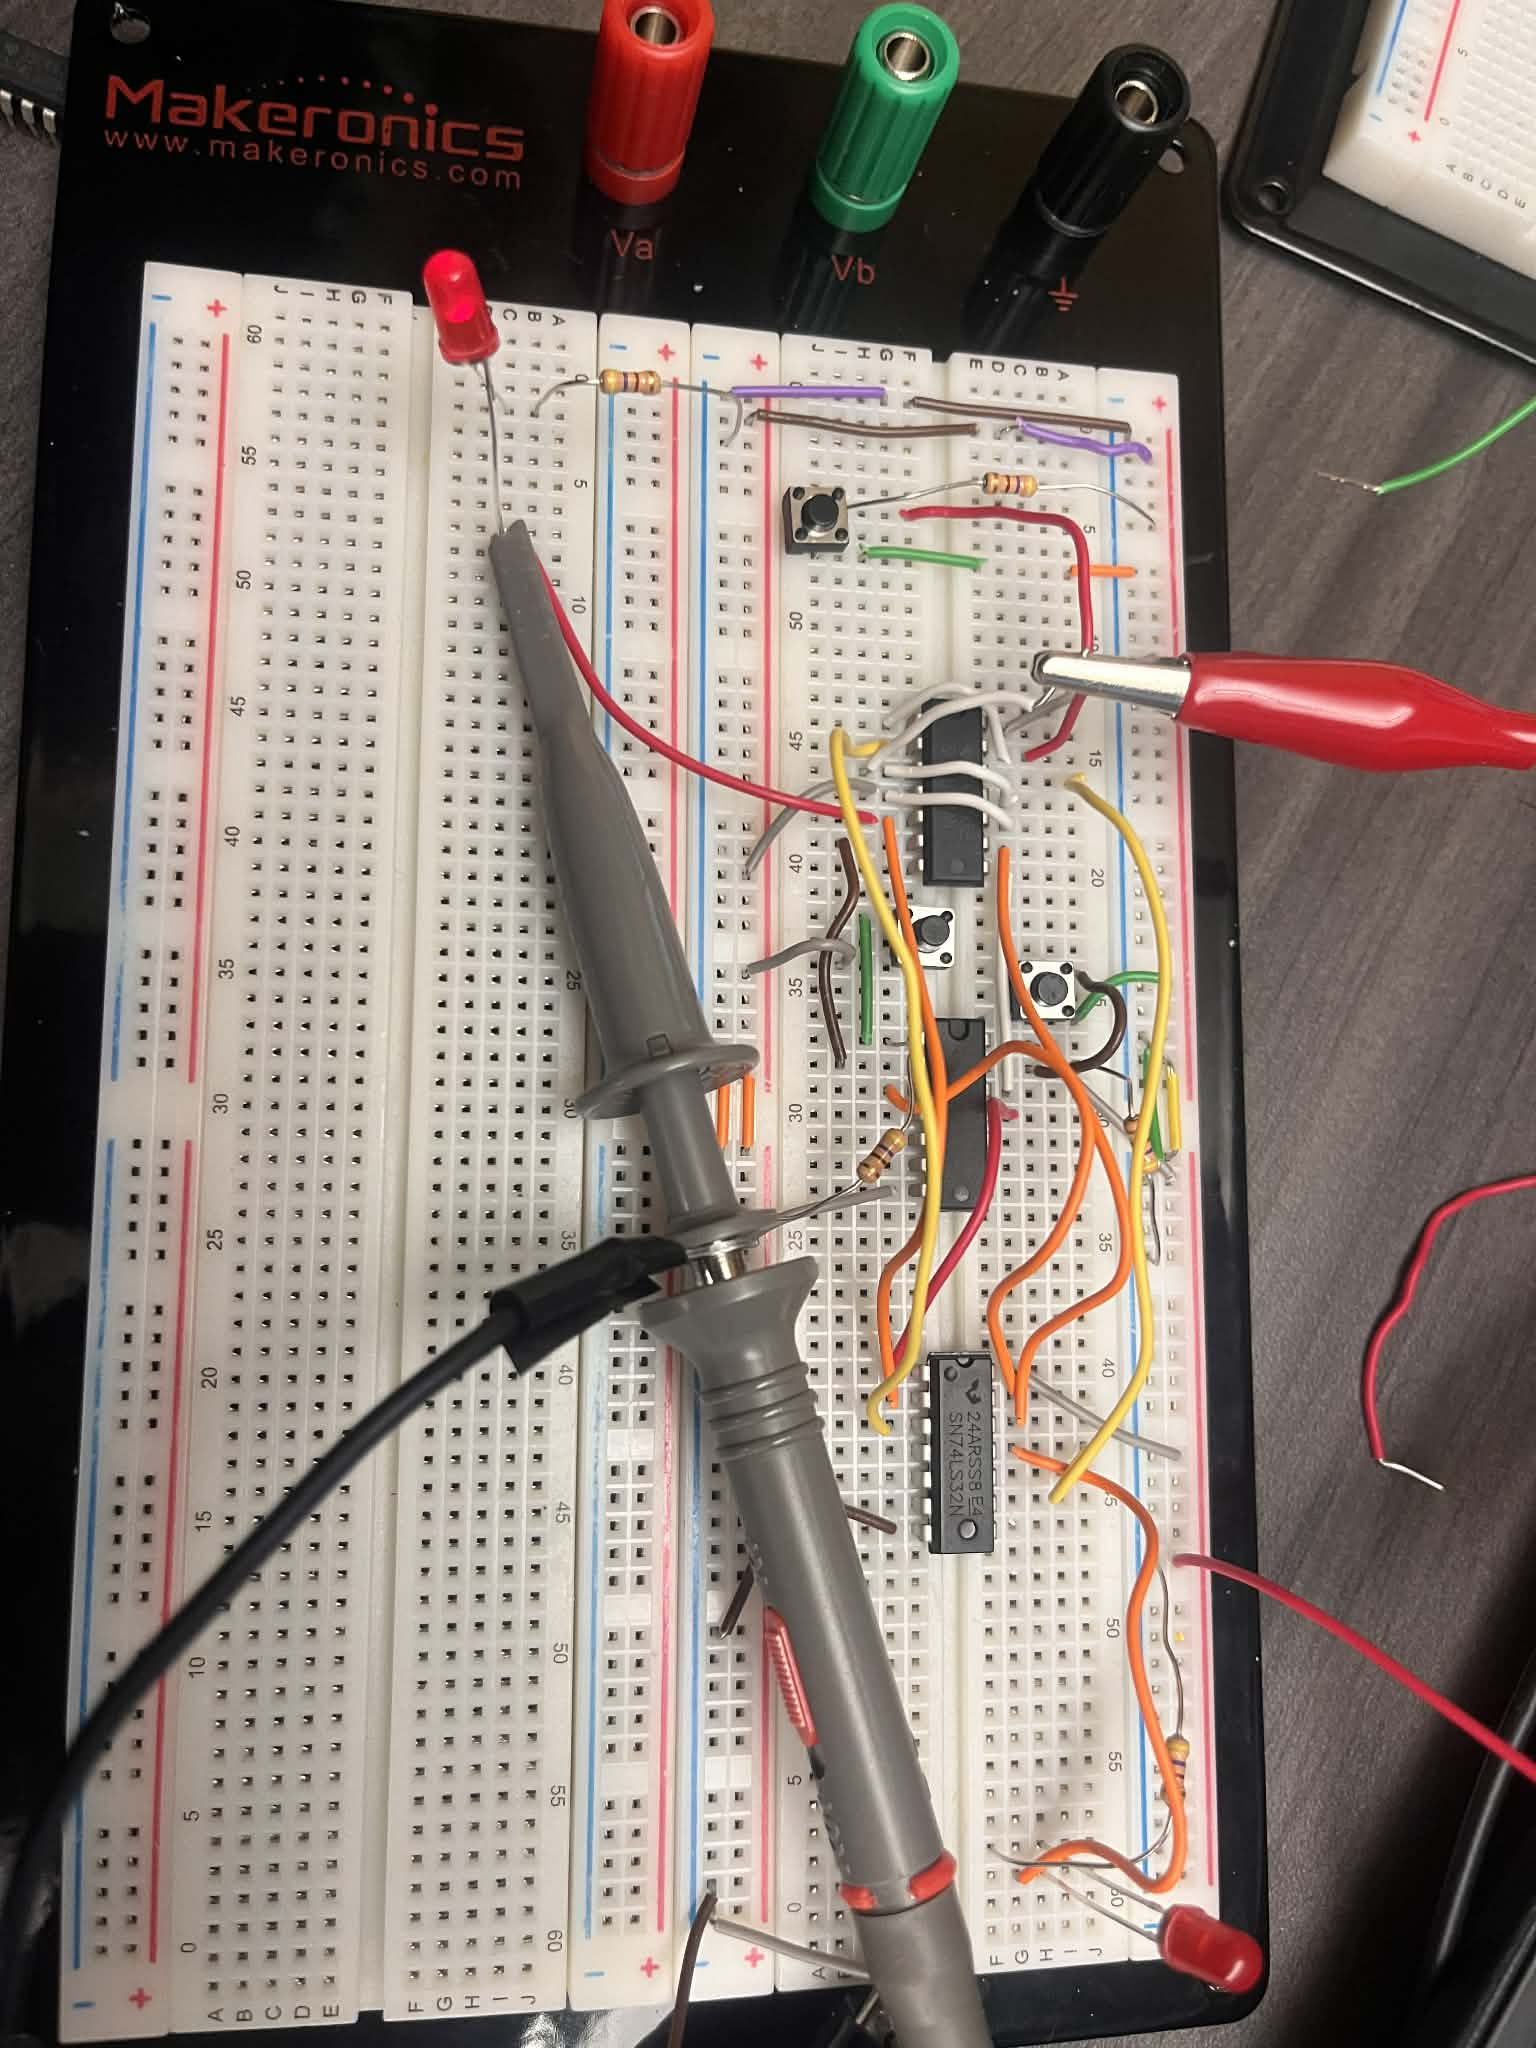
\includegraphics[width=0.75\linewidth]{image5.jpg}
\caption{Overview of the game show circuit implementation on the breadboard, showing the 74LS74 DFF IC, combinational logic wiring, oscilloscope probe, and LED outputs.}
\end{figure}

\begin{figure}[H]
\centering
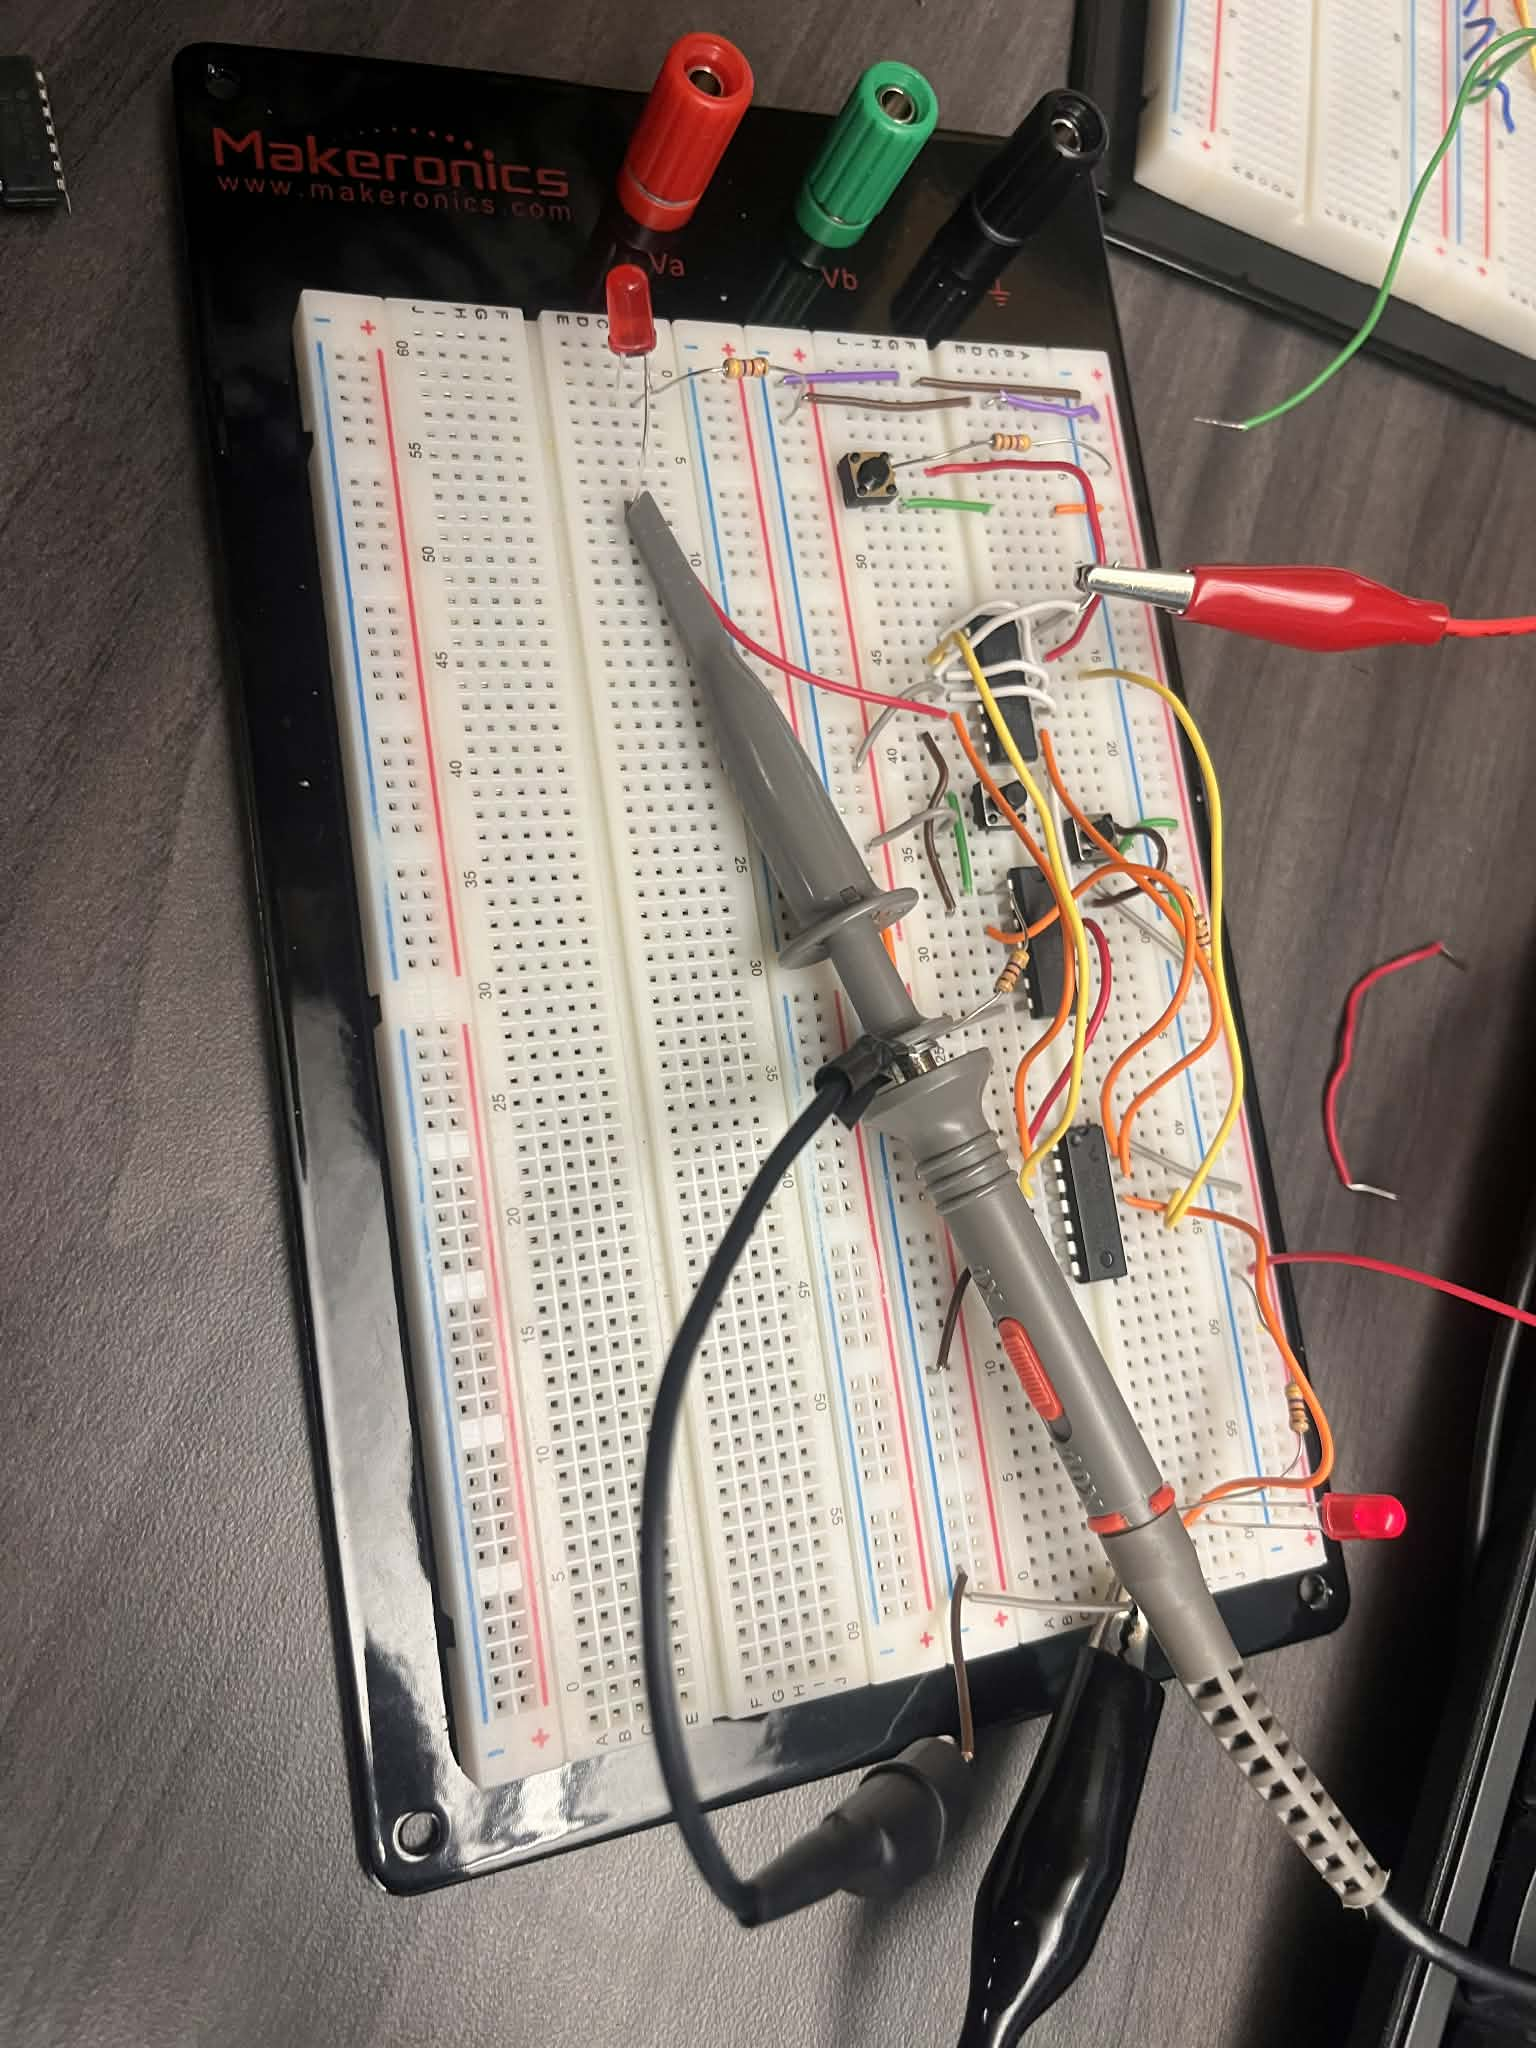
\includegraphics[width=0.75\linewidth]{image3.jpg}
\caption{Circuit in the wait state (State A) after reset is asserted. Both LEDs are off, confirming $Q_1Q_0 = 00$.}
\end{figure}

\begin{figure}[H]
\centering
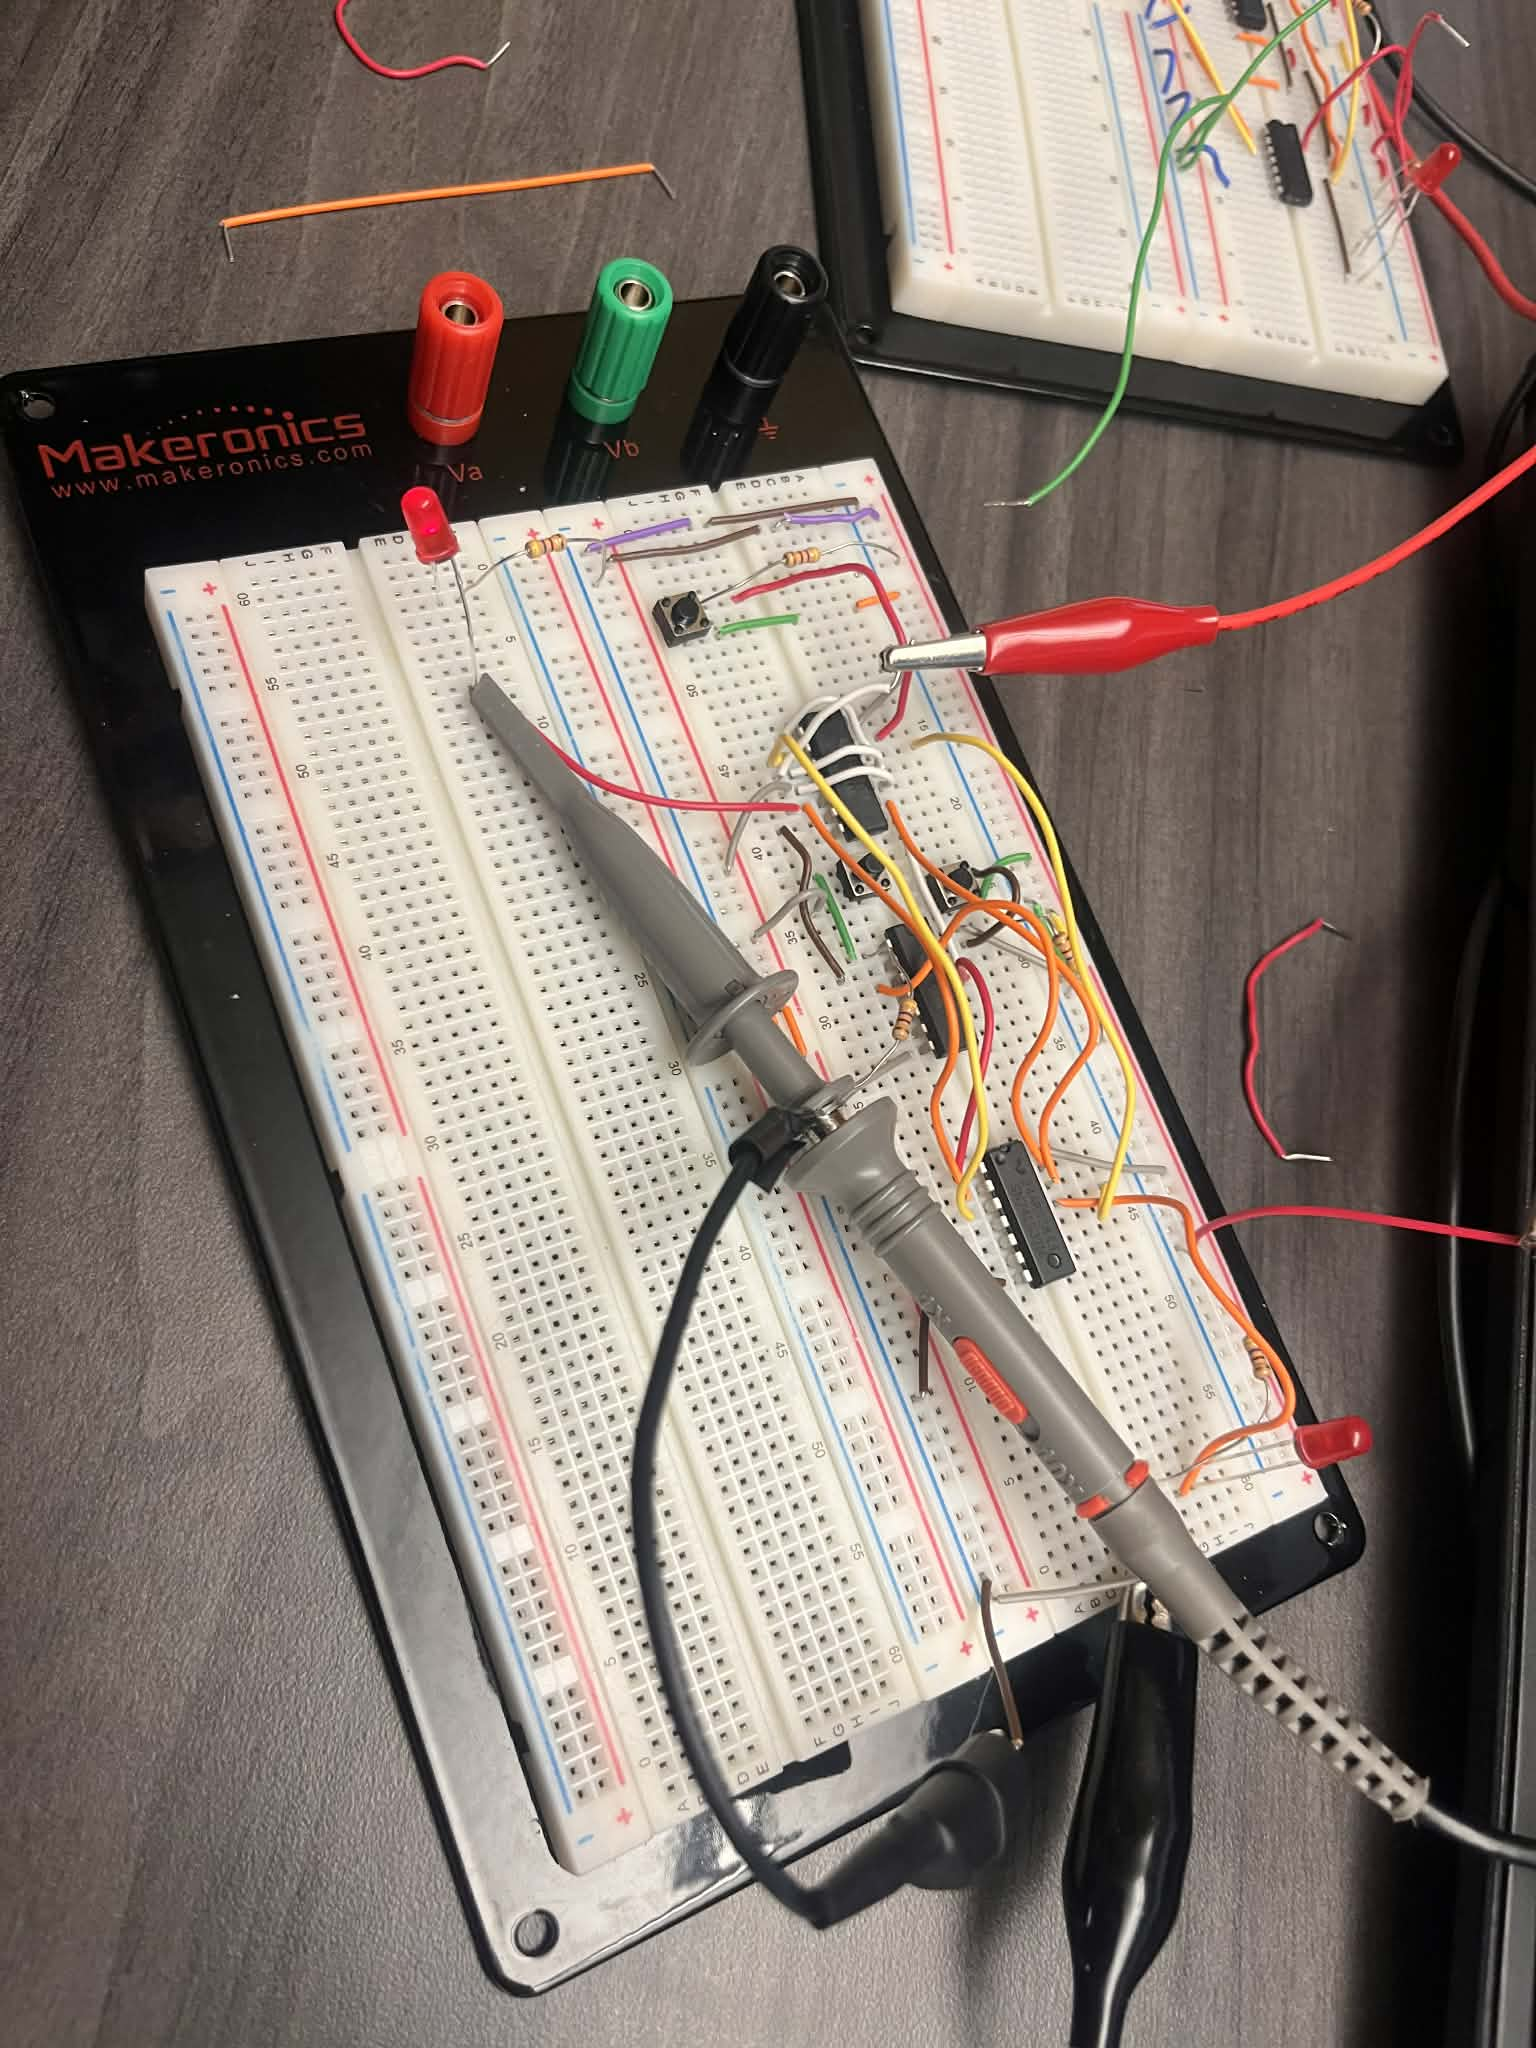
\includegraphics[width=0.75\linewidth]{image1.jpg}
\caption{Testing the circuit: wait state verified with oscilloscope probe connected to monitor the clock signal.}
\end{figure}

\begin{figure}[H]
\centering
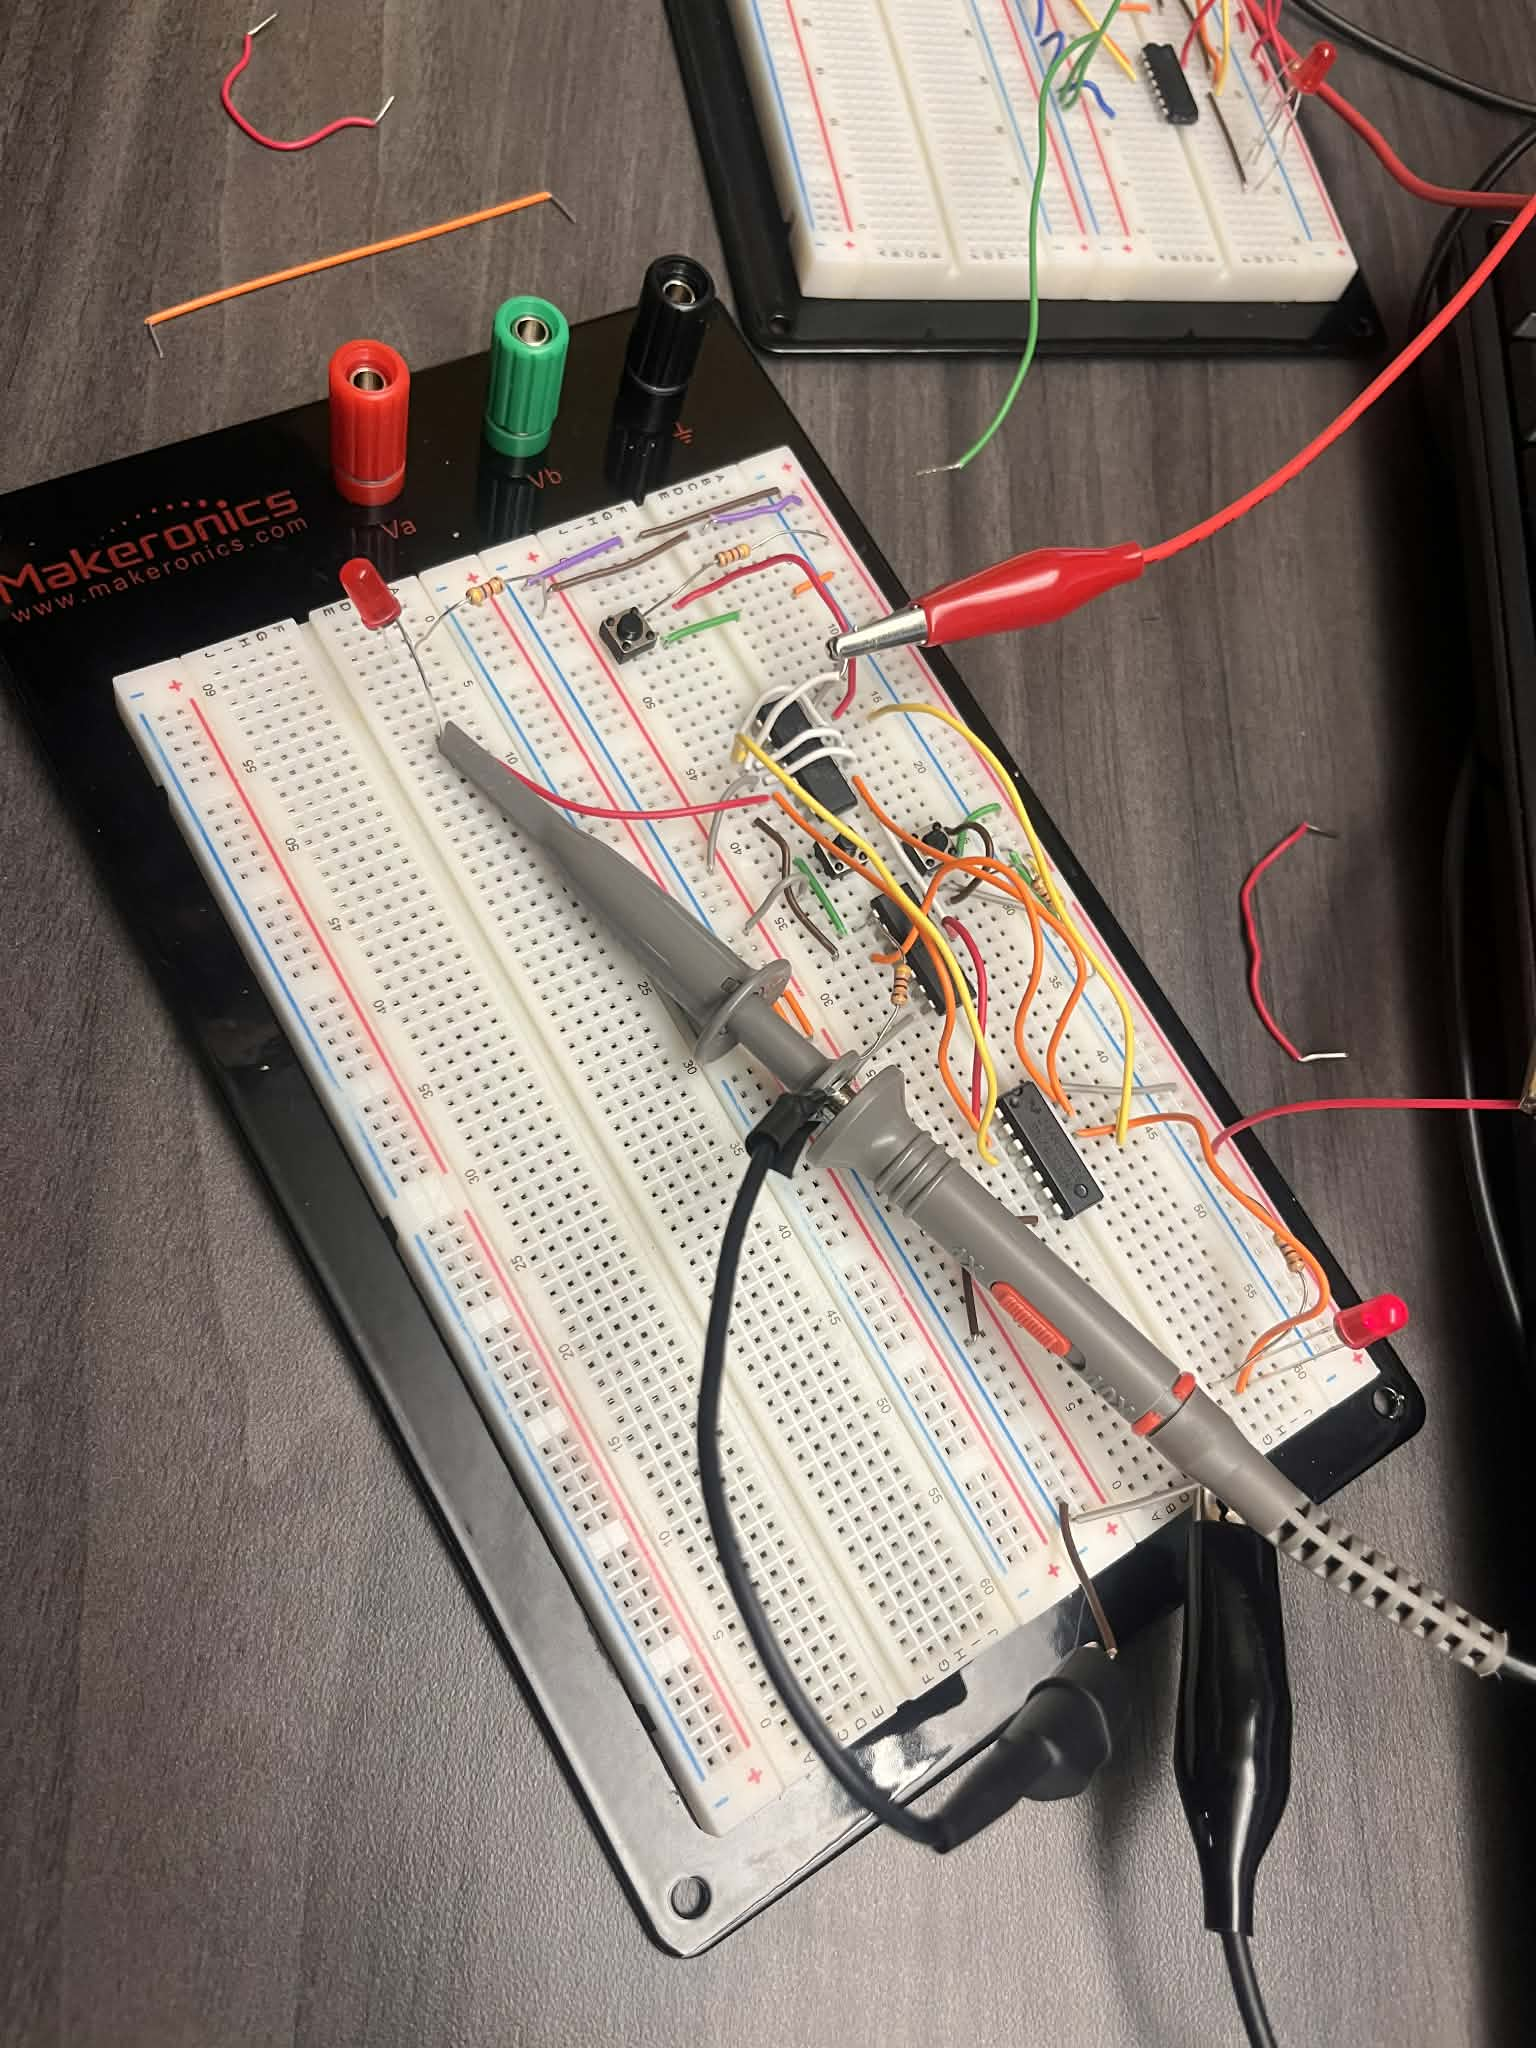
\includegraphics[width=0.75\linewidth]{image2.jpg}
\caption{Contestant 0 wins: after asserting $X_0$, LED0 turns on (State B, $Q_1Q_0 = 01$). The circuit remains locked in this state even when $X_1$ is subsequently asserted.}
\end{figure}

\begin{figure}[H]
\centering
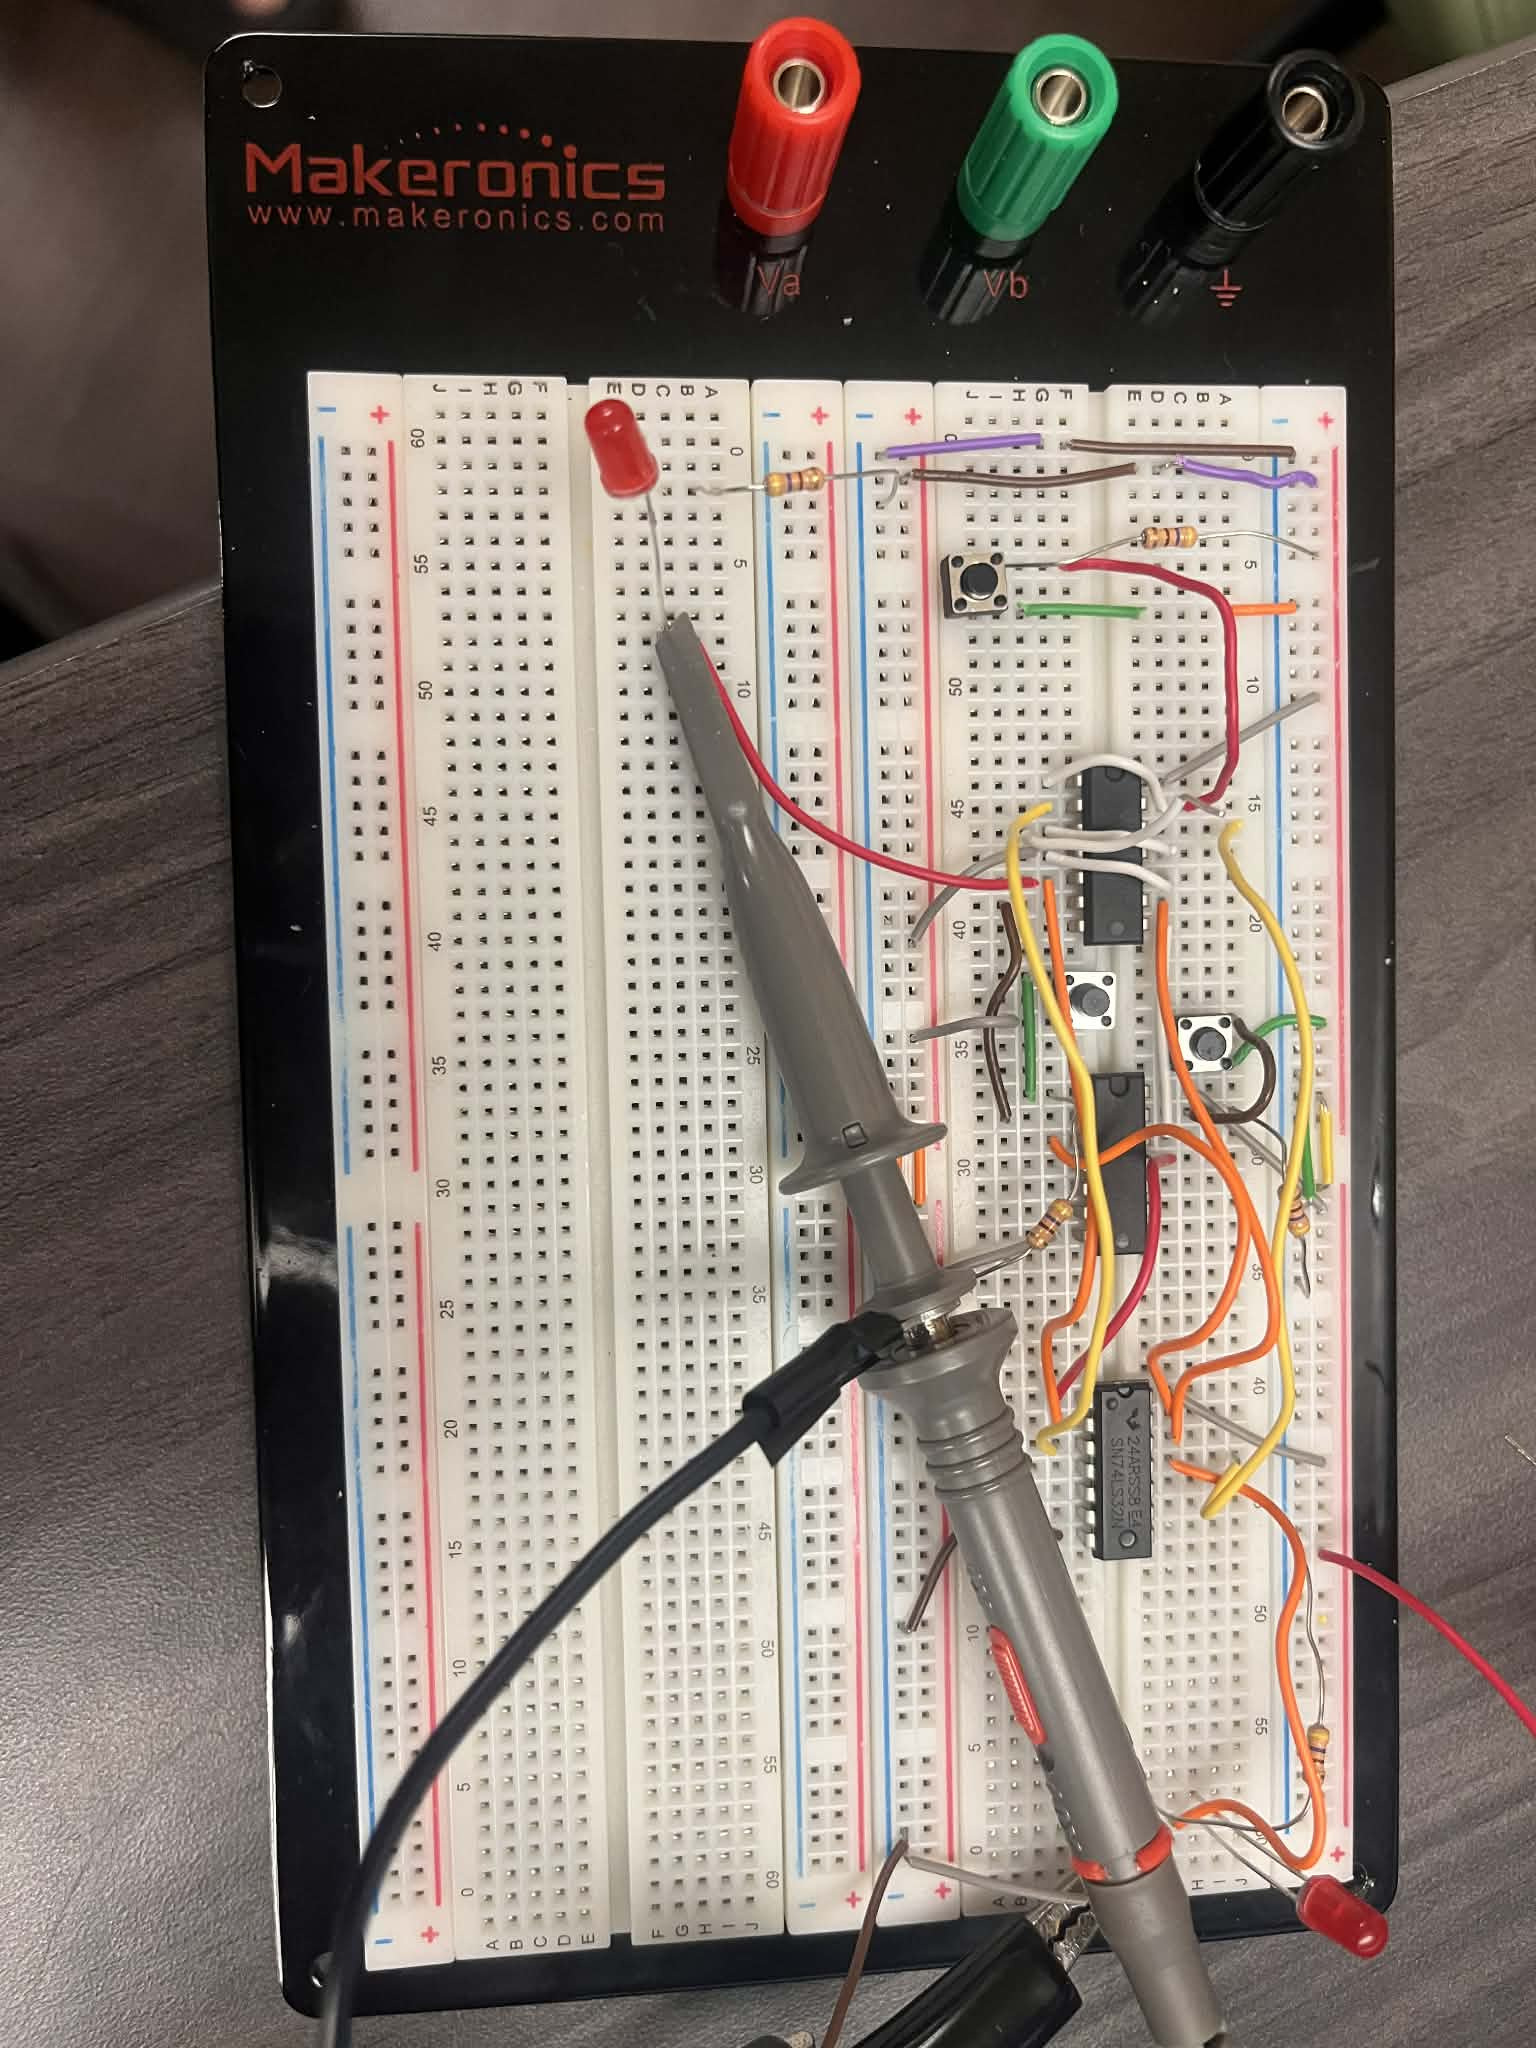
\includegraphics[width=0.75\linewidth]{image4.jpg}
\caption{Contestant 1 wins: after resetting and asserting $X_1$, LED1 turns on (State C, $Q_1Q_0 = 10$). The circuit remains locked in this state regardless of further input.}
\end{figure}

\section{Discussion}

The circuit behaved as expected during testing. After asserting reset, both LEDs were off, confirming the circuit was in the wait state. When contestant 0's button was pressed, LED0 turned on and remained on even after contestant 1's button was pressed subsequently. After resetting and pressing contestant 1's button first, LED1 turned on and stayed on regardless of contestant 0's input. This confirms the locking behavior designed into the state machine.

The results were consistent with our expectations from the state transition table and excitation equations. The symmetry between the two excitation equations ($D_0 = Q_0 + X_0 \cdot \overline{Q_1}$ and $D_1 = Q_1 + X_1 \cdot \overline{Q_0}$) reflects the symmetric design of the circuit, where each contestant's path to winning is identical in structure. The function generator provided a stable clock signal, which was verified on the oscilloscope.

\section{Conclusion}

In this lab, we designed and implemented a sequential game show circuit using D flip-flops. The circuit correctly determines which contestant rings in first and locks the result until reset. We derived the excitation equations using Karnaugh maps, implemented the combinational logic with AND, OR, and inverter gates feeding into a 74LS74 DFF IC, and used a function generator for clocking. The lab reinforced our understanding of sequential circuit design, including state transition tables, excitation equations, and the practical considerations of clocking and resetting flip-flop based circuits.

\end{document}
